\documentclass[14pt]{moderncv}
\usepackage{hyperref}
\usepackage[scale=0.8, top=1cm, bottom=2cm]{geometry}
\usepackage[utf8]{inputenc}
\usepackage{tikz}
\usepackage[a4paper, total={6.5in, 10.5in}]{geometry}
\usepackage{graphicx}
\usepackage{wasysym}
\usepackage{fontawesome}
\usepackage{bbding}
\usepackage[inline]{enumitem} 
\newcommand\sbullet[1][.5]{\mathbin{\vcenter{\hbox{\scalebox{#1}{$\bullet$}}}}}
\moderncvtheme[black]{classic} 
\pagestyle{empty}
\begin{document}
\makecvtitle
\begin{minipage}{0.5\textwidth} 
\begin{flushleft}
    \textcolor{blue}{\Large Sivaprasad Omanakuttan}
\end{flushleft}
 % Required for vertically aligning minipages
	\vspace{-4pt}
	\color{Blue}
	% The first parameter is the FontAwesome icon name, the second is the box size and the third is the text
	% Other icons can be found by referring to fontawesome.pdf (supplied with the template) and using the word after \fa in the command for the icon you want
\textcolor{blue}{\phone}{\hspace{0.15cm} +15055859013}   \\                % optional, remove / 
\textcolor{blue}{\emailsymbol}\href{mailto:somanakuttan@unm.edu}{\hspace{.2cm}somanakuttan@unm.edu} \\   
\textcolor{blue}{\faTwitter} \href{https://twitter.com/SivaprasadOman1}{\hspace{0.15cm}@SivaprasadOman1}\\
\textcolor{blue}{\faGithub} \href{https://github.com/somanakuttan}{\hspace{0.15cm} Github}\\
\textcolor{blue}{\faLinkedin} \href{https://www.linkedin.com/in/sivaprasad-omanakuttan-b26971227/}{\hspace{0.15cm} LinkedIn}\\
\textcolor{blue}{\faGooglePlus} \href{https://scholar.google.com/citations?user=4_fuQdUAAAAJ&hl=en}{\hspace{0.15cm}Google Scholar}
                       % optional, remove / comment the line if not wanted
%
% https://tex.stackexchange.com/questions/172191/skype-icon-in-the-cv-template

     





	
\end{minipage}
\begin{minipage}{0.5\textwidth} 
	\vspace{-\baselineskip} % Required for vertically aligning minipages
\vspace{.3cm}
   \\\\ 	
\textcolor{blue}{About me} I am interested in quantum computing
and quantum information theory. One of the fundamental questions of interest to me is to build a fault tolerant quantum computer. To understand this I use techniques of quantum control, Rydberg dressing, error mitigation, AMO Physics, quantum walk etc.
% Last name
	
  



\end{minipage}
\\\\



\begin{tikzpicture}
\draw (-11,2) -- (5,2);
\node at (-10,2.25) {\textcolor{gray}{Education}};
\draw (-11,2.5) -- (5,2.5);
\end{tikzpicture}\\


\begin{minipage}{0.12\textwidth} 
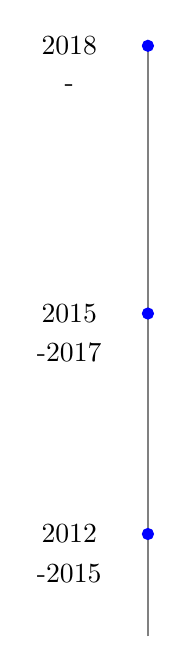
\begin{tikzpicture}

\node at (-2.5,8) {2018};
\node at (-2.5,7.5) {-};
\node at (-2.5,4.6) {2015};
\node at (-2.5,4.1) {-2017};
\node at (-2.5,1.8) {2012};
\node at (-2.5,1.3) {-2015};


\draw[gray, thick] (-1.5,.5) -- (-1.5,8);
\filldraw[blue] (-1.5,8) circle (2pt) node[anchor=west]{};

\filldraw[blue] (-1.5,4.6) circle (2pt) node[anchor=west]{};

\filldraw[blue] (-1.5,1.8) circle (2pt) node[anchor=west]{};
\end{tikzpicture}
\end{minipage}
\begin{minipage}{0.8\textwidth}
\textcolor{blue}{PhD Theoretical Physics, CQuIC UNM}\\
Focus: Quantum computing, quantum information processing, Quantum error Correction, AMO Physics\\
Thesis: Studying how spin systems can be potential candidate for quantum computation (In progress)\\
Supervisor: \href{https://cquic.unm.edu/research/research-groups/deutsch-research-group/index.html}{Prof. Ivan H Deutsch}\\\\
\textcolor{blue}{MSc Indian Institue of Technology,Madras}\\
Focus: Quantum information, Quantum chaos, Combinatorics, Quantum walk\\
Thesis: Investigating the power of discrete time Quantum walk for quantum information and other interesting physical problems\\
Supervisor: \href{https://sites.google.com/view/arulakshminarayan/home}{Prof. Arul Lakshminarayan}\\\\
\textcolor{blue}{BSc Physics Sacred Heart College, Thevara}\\
Thesis: Studied various side effects of nuclear radiation to human health and environment due to radioactive pollution.
\end{minipage}\\

\vspace{.1 in}

\begin{tikzpicture}
\draw (-11,2) -- (5,2);
\node at (-9,2.25) {\textcolor{gray}{Employment History }};
\draw (-11,2.5) -- (5,2.5);
\end{tikzpicture}\\


\begin{minipage}{0.12 \textwidth} 
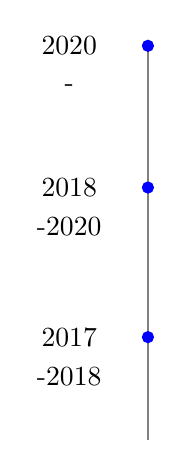
\begin{tikzpicture}
\node at (-2.5,8) {2020};
\node at (-2.5,7.5) {-};
\node at (-2.5,6.2) {2018};
\node at (-2.5,5.7) {-2020};
\node at (-2.5,4.3) {2017};
\node at (-2.5,3.8) {-2018};

\draw[gray, thick] (-1.5,3) -- (-1.5,8);
\filldraw[blue] (-1.5,8) circle (2pt) node[anchor=west]{};
\filldraw[blue] (-1.5,6.2) circle (2pt) node[anchor=west]{};
\filldraw[blue] (-1.5,4.3) circle (2pt) node[anchor=west]{};
\end{tikzpicture}
\end{minipage}
\begin{minipage}{0.88\textwidth}
\textcolor{blue}{Research assistant at University of New Mexico}\\
Working on projects related to quantum information, quantum computation, and atomic physics under the supervision of \href{https://cquic.unm.edu/research/research-groups/deutsch-research-group/index.html}{Prof. Ivan H Deutsch}
\\

\textcolor{blue}{Teaching assistant at University of New Mexico}\\
Teaching assistant for  Quantum Optics, Quantum mechanics, Electromagnetism and classical mechanics\\

\textcolor{blue}{Project associate at Indian Institute of Technology Madras }\\
Worked on projects related to quantum information and quantum chaos under the supervision of  \href{https://sites.google.com/view/arulakshminarayan/home}{Prof. Arul Lakshminarayan} and Dr. Prabha Mandayam.
\end{minipage}\\\\
\newpage

\begin{tikzpicture}
\draw (-11,2) -- (5,2);
\node at (-9.8,2.25) {\textcolor{gray}{Publications}};
\draw (-11,2.5) -- (5,2.5);
\end{tikzpicture}\\

\begin{minipage}{.95\textwidth}
\begin{itemize}
\item {\textcolor{blue}{ Spin squeezed GKP codes for quantum error correction in atomic ensemble} \textbf{S O}, and Dr. Tyler Volkoff (in preparation)} 

  \item{\textcolor{blue}{Creating entangling Qudit gates using Quantum optimal control}  \textbf{S O}, Anupam Mitra, Michael J. Martin and Ivan H. Deutsch (in preparation)}  
  \item{\textcolor{blue}{Practical and fundamental limits of neutral atom entanglement using Rydberg dressing}  Anupam Mitra, \textbf{S O}, Prof. Grant W. Biedermann , Michael J. Martin and Ivan H. Deutsch (arXiv preprint arXiv:2205.12866)}  
\item \textcolor{blue}{Article:\href{https://arxiv.org/abs/2106.13705}{ Quantum Optimal Control of Nuclear Spin Qudecimals in \textsuperscript{87}Sr}} \textbf{S O}, Anupam Mitra, Michael J. Martin and Ivan H. Deutsch, arXiv preprint arXiv:2106.13705 (accepted to PRA letters).
\item \textcolor{blue}{Article: \href{https://arxiv.org/abs/2110.02286}{Flavor isospin waves in one-dimensional axisymmetric neutrino gases}} Huaiyu Duan, Joshua D Martin and \textbf{S O}, arXiv preprint arXiv:2110.02286, 2021 (accepted to PRD).
\item \textcolor{blue}{Article: \href{https://journals.aps.org/pre/abstract/10.1103/PhysRevE.103.012207}{Quantum walks with quantum chaotic coins: Loschmidt echo, classical limit, and thermalization}} \textbf{S O} and Arul Lakshminaryan Phys. Rev. E 103, 012207.
\item \textcolor{blue}{Article:\href{https://journals.aps.org/pre/abstract/10.1103/PhysRevE.99.062128}{ Out-of-time-ordered correlators and quantum walks}} \textbf{S O} and Arul Lakshminaryan Phys. Rev. E 99, 062128.
\item \textcolor{blue}{Article:\href{https://iopscience.iop.org/article/10.1088/1751-8121/aad50c/meta}{ Quantum walk on a toral phase space}} \textbf{S O}  and Arul Lakshminaryan J. Phys. A: Math. Theor. 51 385306.\\
\end{itemize}
\end{minipage}




\begin{tikzpicture}
\draw (-11,2) -- (5,2);
\node at (-9.4,2.25) {\textcolor{gray}{Ongoing projects}};
\draw (-11,2.5) -- (5,2.5);
\end{tikzpicture}\\


\begin{minipage}{.95\textwidth}
\begin{itemize}
  
\item \textcolor{blue}{Quantum error correction in Spin systems}\\
Goal: To understand how error correction can be practically achieved in spin systems
Collaborators: Prof. Milad Marvian, Dr. Jonathan Gross, and Prof. Ivan H Deutsch


\item\textcolor{blue}{Quantum control using Magnetic dressing}\\
Goal: Use the unique property of nulear spin vs electronic spin in alkalne earth elements for quantum control\\
Collaborators: Dr. Michael J Martin, and Prof. Ivan H Deutsch

\item\textcolor{blue}{Error mitigation with qudits and dynamical decoupling}\\
Goal: Understanding various applications of error mitigation for quantum computation.\\
Collaborator: \href{http://www.unm.edu/~mmarvian/}{Prof. Milad Marvian} 

\item\textcolor{blue}{Hamiltonian control}\\
Goal: Hamiltonian engineering using underlying Lie algebra\\
Collaborator: \href{https://sites.google.com/view/pablopoggi/}{Dr. Pablo Poggi}

\item\textcolor{blue}{Creating high fidelity entangler for qubits using Rydberg interaction}\\
Goal: High fidelity qubit entanglers in neutral atoms using Rydberg dressing.\\
Collaborators: Sri Datta Vikas Buchemmavari,Yuan-Yu Jau and Prof. Ivan H Deutsch\\

\item\textcolor{blue}{A new measure of scrambling}\\
Goal: Use an new method to understand out of time order correlator for understanding scrambling.\\
Collaborators: Karthik Chinni, Dr. Pablo Poggi, Philip Blocher\\

\end{itemize}

\end{minipage}\\
\newpage

\begin{tikzpicture}
\draw (-11,2) -- (5,2);
\node at (-8.5,2.25) {\textcolor{gray}{Presentations and Posters}};
\draw (-11,2.5) -- (5,2.5);
\end{tikzpicture}\\

\begin{minipage}{.95\textwidth}
\begin{itemize}
    \item \textcolor{blue}{Talks on Quantum Optimal Control for qudit entanglers }\\
     March Meeting 2022\\
     DAMOP22\\
    \item \textcolor{blue}{Talks on Quantum Optimal Control of Nuclear Spin Qudecimals }\\
     APS four corners meeting 2021\\
APS March Meeting 2021\\
\href{https://indico.frib.msu.edu/event/31/overview}{YQIS 2021}\\
\href{https://meetings.aps.org/Meeting/DAMOP21/Session/S08.8}{DAMOP21}
\item Poster on Quantum walk with deterministic dynamical systems,
\href{http://physics.unm.edu/SQuInT/2020/poster_abstracts.php}{SQuInT 2020}
\item Poster on Implementing qudit quantum logic gates on nuclear spins in Strontium-87 atoms, \href{http://physics.unm.edu/SQuInT/2021/poster_abstracts.php}{SQuInT 2021}\\
\end{itemize}
\end{minipage}


\begin{tikzpicture}
\draw (-11,2) -- (5,2);
\node at (-8.6,2.25) {\textcolor{gray}{Awards and Achievements}};
\draw (-11,2.5) -- (5,2.5);
\end{tikzpicture}\\


\begin{minipage}{0.10\textwidth} 
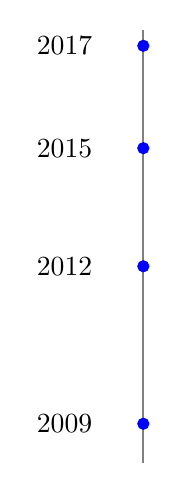
\begin{tikzpicture}
\node at (-2.5,6.8) {2017};
\node at (-2.5,5.5) {2015};
\node at (-2.5,4) {2012};
\node at (-2.5,2) {2009};\\\\

\draw[gray, thick] (-1.5,1.5) -- (-1.5,7);
\filldraw[blue] (-1.5,6.8) circle (2pt) node[anchor=west]{};
\filldraw[blue] (-1.5,5.5) circle (2pt) node[anchor=west]{};
\filldraw[blue] (-1.5,4) circle (2pt) node[anchor=west]{};
\filldraw[blue] (-1.5,2) circle (2pt) node[anchor=west]{};
\end{tikzpicture}
\end{minipage}
\hspace{0.3cm}
\begin{minipage}{0.8\textwidth}
Secured an All India Rank of 99 (percentile: 99.11)  for entrance for post graduate level students in physics\\

Secured an All India Rank of 471 in JAM conducted
for admissions for entrance for graduate level students in physics.\\

An INSPIRE fellow, the Indian Government's scholarship program to best outgoing students graduating from higher
secondary school (Top 1\%) in the science sector.\\

Awarded National Means cum -Merit Scholarship (NMMS), which is given given to selected students from class IX -XII.

\end{minipage}\\\\












\begin{tikzpicture}
\draw (-11,2) -- (5,2);
\node at (-10,2.25) {\textcolor{gray}{IT skills}};
\draw (-11,2.5) -- (5,2.5);
\end{tikzpicture}\\

\begin{minipage}{1\textwidth} 
\begin{itemize}
    \item C++, Python, Mathematica, Julia, Matlab
    \item LATEX, Microsoft Office
\end{itemize}\\


\end{minipage}\\

\vspace{.2cm}

\begin{tikzpicture}
\draw (-11,2) -- (5,2);
\node at (-8.7,2.25) {\textcolor{gray}{Relevant Courses Taken}};
\draw (-11,2.5) -- (5,2.5);
\end{tikzpicture}\\

\begin{minipage}{\textwidth} 

\textcolor{blue}{Graduate level courses}
\begin{itemize}
    \item Quantum Mechanics I and II 
    \item Quantum optics I and II
    \item Quantum Error Correction
    \item Quantum Computation
    \item Quantum information Theory
    \item Quantum Machine learning (an online course of study offered by University of TorontoX, an online learning initiative of University of Toronto.)
    \item Statistical Mechanics
    \item Electrodynamics
\end{itemize}


\end{minipage}





\end{document}